\chapter{Design}

\section{System Architecture}

\begin{figure}[h]
  \label{overviewfigure}
  \centering
  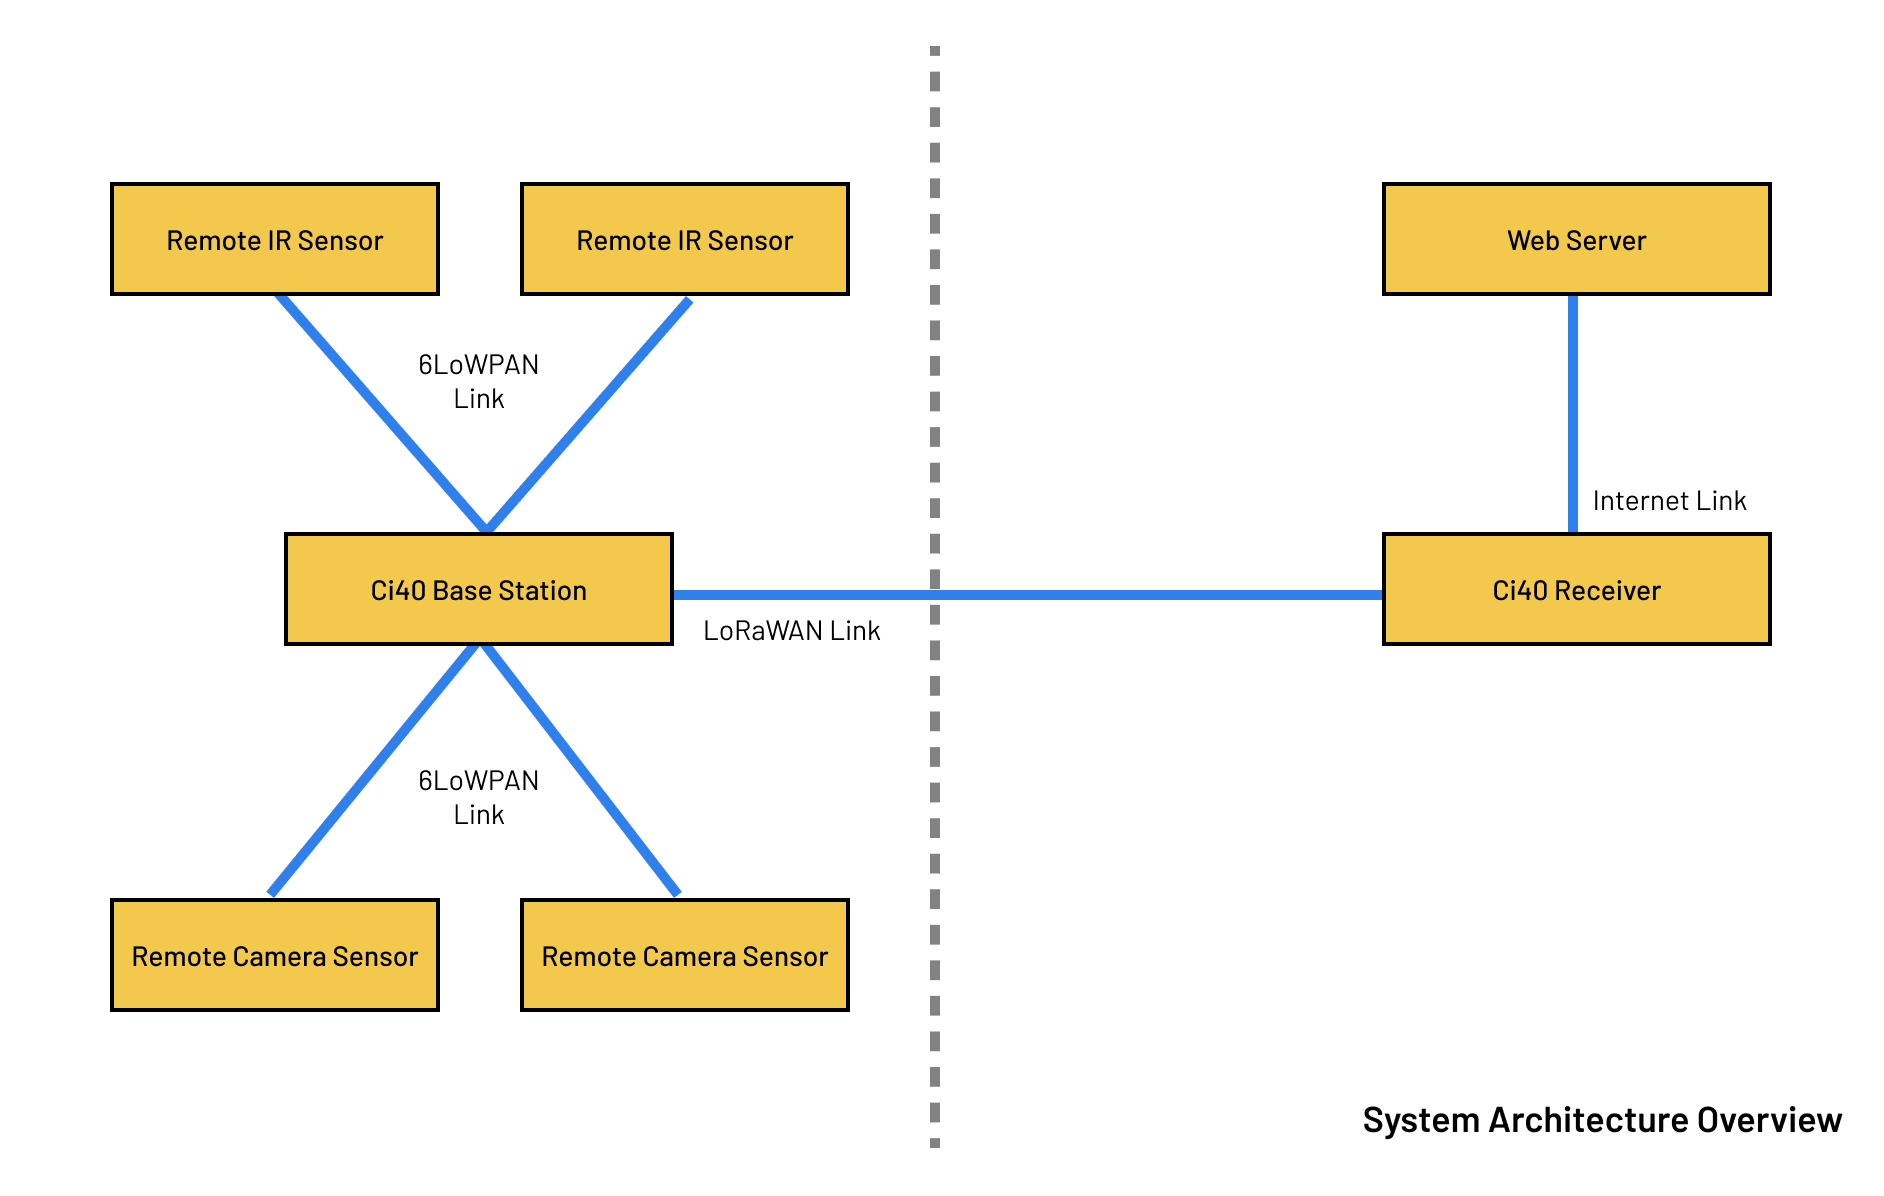
\includegraphics[width=\textwidth]{systemoverview}
  \caption{System architecture overview, showing how the high-level components of the system are connected.}
\end{figure}

Figure~\ref{overviewfigure} shows the connections between the high-level
components in the system, including the sensor deveices and the base
stations, as well as the web server used to store and retrieve data.

\subsection{Base Station}
As previously mentioned in the requirements, the base station is a
\textit{Creator Ci40 \acrshort{iot} Hub} device~\cite{creatorci40}. It is a
development board that is highly specialised for rapidly building
\acrlong{iot} applications, due to its abundance of sockets, pins and radios
for \acrshort{io}.

\subsubsection{Hardware Design Features}

The Ci40 board includes a \gls{6lowpan} radio, which is crucial in allow it
to conduct two-way communication with nearby sensing devices at a reasonably
high data rate. The main drawback is the range, which is typically a couple
of tens of meters~\cite{culler20096lowpan}. However, this is perfect for
communicating with the nearby sensor devices, which won't be too far away
from the base station in the first place, and there is also the potential to
use a mesh-style network, where communication might happen via one or more
intermediary nodes. However, this would require sensor devices to be
constantly active, thus preventing them from entering a lower power state and
resulting in a much higher power usage.

\subsubsection{Software Design}
The base station provides a couple of very important tasks. Firstly, it acts
as the main router, or coordinator, for nearby motion detector and camera
pairs. It receives a motion alert from the motion sensor and sends a command
to the related camera to capture an image. This program would also need to
keep a list of sensor pairs, to ensure each command gets sent to the correct
sensor.

In addition to this, the base station runs a program to process incoming
images from the camera sensors and calculates the count and species of any
wildlife in the photo. Since this is an image recognition problem, it was
decided that the best solution would be to use a convoluted neural network,
trained on a dataset of similar images, to estimate to a reasonable accuracy
the species of wildlife in the image. However, since the Ci40 board uses a
32-bit processor architecture, it makes running neural networks a little more
difficult, since most frameworks will only support 64-bit processors, as the
larger word length results in larger computations being made possible.

Finally, the base station needs to act as a \gls{lorawan} transmitter, to
send the count data to an Internet-connected base station, which can then in
turn upload the results to the web server. So, the base station is running
three programs at the same time to deal with different tasks. All of the code
that deals with the \gls{6lowpan} connection or \gls{lorawan} connection is
written in either C or Python, and uses the \textit{LetMeCreate} library
provided by the board manufacturer to increase ease of development.

\subsection{Remote Sensors}

\unsure[inline]{include graphic of camera pairs in trees etc?}

The system also utilises a set of remote sensors that wirelessly connect with
the base station using a \gls{6lowpan} connection. There's two kinds of
sensors being used in the system, motion detector sensors and camera sensors.
Both sensors use the same base board, a \textit{MikroElektronika}
\gls{6lowpan} Click Board~\cite{mikroeclick}, with either a camera or motion
detector attachment.

\subsubsection{Hardware Design}

\todo[inline]{Include image of 6LoWPAN clicker}
The \textit{MikroElektronika} \gls{6lowpan} Click Board, as previously
mentioned, runs a \acrfull{rtos} called \gls{contiki}. According to the
\gls{contiki} project website~\cite{contiki}, it is ideal for low-power
\acrshort{iot} projects since it supports the full \acrshort{ipv4} and
\acrshort{ipv6} networking suites, as well a being able to run on ``tiny
systems, only having a few kilobytes of memory available''. \textit{Creator},
the manufacturers of the Ci40 base station, provide a toolchain for writing
programs to the click board, as well as abstraction libraries for network and
sensor interfaces~\cite{letmecreate}.

Creator also provide a set of guides to help set up and write programs to the
flash memory onboard the clicker device~\cite{clickersetupguide}, which have
proven invaluable. Code is written in a slightly modified version of the C
programming language; the main difference being that all of the code runs in
process threads that can be suspended, resumed and interrupted.

\subsubsection{Communication}
The remote sensors communicate with the base station using
\acrshort{json}-encoded strings sent via \acrshort{tcp} over \gls{6lowpan}. A
set of commands are defined and recognised by the sensors and the base
station server alike, to allow messages to be sent that are both brief and
human-readable, which is invaluable when debugging. The messages take a form similar to this:

\begin{verbatim}
  { "device_id": 1, "command": "heartbeat" }
\end{verbatim}

A unique \texttt{device\_id} is provided by every sensor to identify itself
to the base station server, and on its first connection it will also provide
a \texttt{pair\_id} which tells the server which unique camera/motion
detector pair the device belongs to. Each of these are provided to the sensor
program at compile time, using environment variables.~\improvement{Add list
of commands?}

\subsubsection{Motion Detector Sensor}
\todo[inline]{include image of motion click}
The motion detector sensor uses the \gls{6lowpan} Click board described
above, with a \textit{MikroElektronika} Motion Click
device~\cite{motionclick} integrated onto the board using the
``\gls{mikrobus}'' port. According to the product page~\cite{motionclick}, it
has a range of up to four metres which is probably not sufficient for real
world usage. However, for prototyping purposes, it is perfect because of the
ease of integration, thanks to the aforementioned \textit{LetMeCreate}
library~\cite{letmecreate}.

The code runs in a continuous loop, that yields the main thread until it is
resumed by an event interrupt. This event could be one of:

\begin{itemize}
  \item a timer expiring,
  \item a \acrshort{tcp} event (received packets, lost connection, et cetera),
  \item a motion detection event received from the motion sensor.\unsure{any
  other events?}
\end{itemize}

For the prototype version of this sensor, the code sends a ``heartbeat''
command to the base station every twenty seconds, for debugging purposes. But
in a production version, the processor would only be be interrupted by
\acrshort{tcp} events or by motion detection events, as this would result in
fewer interrupts over time and thus reduce the power usage of the device. The
development version of the program also makes use of a debug server running
on the base station. The clicker board does not always have a serial
output available, so printing to console (i.e., using the \texttt{printf()}
function) does not work. Therefore, Contiki includes a \texttt{PRINTF} macro
that sends the string to a server using \gls{6lowpan}, if available.

\subsubsection{Camera Sensor}

\todo[inline]{include image of camera click}
The camera sensor comprises of the same \gls{6lowpan} Clicker board, but
instead of a motion sensor, there is a \textit{MikroElektronika} Camera Click
board~\cite{cameraclick} installed onto the \gls{mikrobus} port. The board
contains a digital camera sensor which, according to the specification page,
has a maximum resolution of 640 by 480 pixels. It also contains an extra
microcontroller, which ``outputs the camera image to the target board
microcontroller through the \gls{mikrobus} SPI interface''. Essentially, it
appears to transform the raw data stream from the camera into a data stream
that can be sent using \acrfull{spi} to the `target' board (in this case, the
\gls{6lowpan} clicker). However, a lot of the board's inner
workings\textemdash save for the board schematics, available on the product
page\textemdash is largely closed-source.

The code examples provided by
\textit{MikroElektronika}~\cite{cameraclickexamples} helped to provide a
little bit of insight into how the camera can be operated. For example, it
provides a list of \glspl{opcode} that the camera click accepts, such as
requesting an image, or getting/setting a register on the camera sensor
itself.

The main objective of the camera sensor is to respond to a message sent from
the base station (over \gls{6lowpan}) commanding it to take a photo and send
the photo back to the base station over the same connection.

\subsection{Web Server}
The web server serves the purpose of storing incoming species counts and
types from any number of base stations, as well as keeping track of the
locations of the base stations and sensors. Since the sensors and devices
don't possess geolocation capabilities, this would be something that a
research team using this solution would have to manually input.

As well as providing a way of uploading and storing this information, the web
server would also have to provide methods of retrieving the data, as well as
displaying the data. To this end, an \acrshort{api} is the best solution for
the problem. Appendix~\ref{app:apispec} shows a copy of the \acrshort{api}
specification that was created before development began on the \acrshort{api}
itself. Specifications are highly important, since they could be used to help
develop comprehensive test suites for the code itself, as well as provided a
solid foundation for any further documentation, for instance documentation
that third parties use to build on top of the \acrshort{api}.

The first stage in building the \acrshort{api} is to model how the data is to
be represented. This is achieved in three stages:

\begin{enumerate}
  \item Work out what entities are to be represented with the API. For this
  project, this ended up being: the base stations, the associated sensor
  pairs, and the readings obtained from the sensor pairs. The web server
  doesn't need to concern itself with how the pairs connect to the base
  stations and to each other, so it is easier to model each motion sensor and
  camera sensor as a single pair.
  \item Construct an entity-relationship diagram, to represent how each of
  the entities listed interact with each other. This also introduces the
  notion of multiplicity; for instance, how many base stations does a sensor
  pair interact with?~\todo{include E-R diagram (and ref here)}
  \item For each entity, deciding what data needs to be stored and accessible
  from the \acrshort{api}. As mentioned earlier, a lot of data is actually
  excluded here since it is only relevant at a lower level. An example of
  data that is deliberately excluded is sensor \acrshort{ipv6} addresses,
  since they're only required by the base station for communication. This is
  also when it would be decided what data is necessary and \textbf{must} be
  included for each instance of the entity, and what data is optional.
  Human-readable names are a good example of this.
\end{enumerate}

From this initial requirements gathering, it is then possible to create an
\acrshort{api} specification, detailing how the \acrshort{api} should react
to certain input. It should be highly detailed, included specifying the
\acrshort{http} response code that would be received under normal conditions.

The entire \acrshort{api} specification is included in
Appendix~\ref{app:apispec} for the reader's perusal.